\section{Χαρακτηριστικά και προεπεξεργασία δεδομένων}

Για την εξαγωγή των χαρακτηριστικών που φαίνονται στο από τα αρχεία ήχουν του σετ δεδομένων, αρχικά τμηματήσαμε κάθε σήμα αρχείου σε frames με μέγεθος 6144 δείγματα. Έπειτα, τα frames αυτά, παραθυροποιήθηκαν με παράθυρο τύπου Hamming, ίσου μεγέθους. Στη συνέχεια, έγινε η εξαγωγή των χαρακτηριστικών στο πεδίο του χρόνου, καθώς και στο πεδίο της συχνότητας.Παράλληλα, έγινε και η εξαγωγή των συντελεστών MFCC έτσι ώστε να είναι εφικτός ο υπολογισμός της διαμόρφωσης της ενέργειας σήματος στα 4 hz. Τα χαρακτηριστικά που εξήχθηκαν είναι 27 και θα αναλυθούν στη συνέχεια. Ως προεπεξεργασία, τα δεδομένα κλιμακοποιήθηκαν έτσι ώστε να έχουν μέσο 0 και τυπική απόκλιση ίση με 1 για κάθε συνιστώσα. Τέλος, δίνουμε την δυνατότητα στον κώδικά μας να εφαρμοστεί και η μέθοδος Principal Component Analysis - PCA,αν αυτή είναι αναγκαία, έτσι ώστε να μειωθούν οι τελικές διαστάσεις των χαρακτηριστικών.Η χρήση της αυτής της μεθόδου, μειώνει τις διαστάσεις σε 10 από τις 27 που έχουμε τώρα αλλά ρίχνει την απόδοση στο 89.72\% , μικρότερη από αυτήν που πετυχαίνουμε εν τέλη όπως θα δούμε στη συνέχεια. 

%pinakas me arxikes kai telikes diastaseis xarakthristikwn
% \begin{center}
% \begin{tabular}{ |c |c| }
% \hline
%  cell1 & cell2 & cell3 \\ 
%  cell4 & cell5 & cell6 \\  
%  cell7 & cell8 & cell9    
%  \hline
% \end{tabular}
% \label{table:1}
% \end{center}

\subsection{Zero Crossing Rate - ZCR}

Είναι ο ρυθμός της αλλαγής προσήμου κατά τη διάρκεια του σήματος, δηλαδή ο ρυθμός με τον οποίο το σήμα αλλάζει από θετικό και αρνητικό και αντίστροφα. Σε κάποιο βαθμό, δείχνει την μέση συχνότητα του σήματος ως εξής:
\begin{equation}
\text{ZCR} = \frac{\sum_{m=1}^{N} |sgn ~x(n) - sgn~x(n-1)| }{2N}
\end{equation}

όπου sgn() η συνάρτηση προσήμου και x(m) το διακριτό σήμα ήχου. Στη γενική περίπτωση, το ZCR για την μουσική είναι αρκετά υψιλότερο από ότι στην φωνή.

% \begin{figure}[H]
% \begin{subfigure}{.5\textwidth}
%   \centering
%   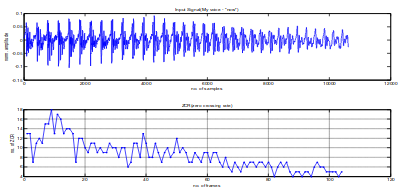
\includegraphics[width=.8\linewidth]{humanvoice.png}
%   \caption{Φωνή}
%   \label{fig:sfig1}
% \end{subfigure}%
% \begin{subfigure}{.5\textwidth}
%   \centering
%   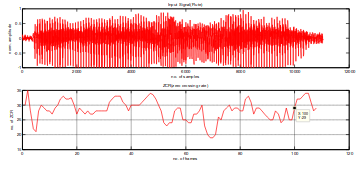
\includegraphics[width=.8\linewidth]{musicinstr.png}
%   \caption{Μουσική}
%   \label{fig:sfig2}
% \end{subfigure}
% \caption{Σήματα φωνής και μουσικής με τα αντίστοιχα ZCR \footnote{Discrimination between Speech and Music signal, Sumit Kumar Banchhor,International Journal of Soft Computing and Engineering (IJSCE)}}
% \label{fig:fig}
% \end{figure}

\subsection{Spectral Centroid - SC}

Το spectral cendroid ή αλλιώς φασματικό κέντρο , όπως αναφέρεται στο Footnote είναι μία μετρική που χρησιμοποιείται ώστε να χαρακτηρίσει ένα φάσμα. Υποδεικνύει πού βρίσκεται το κέντρο του φάσματος. Έχει ισχυρή σύνδεση με την "φωτεινότητα " ενός ήχου δηλαδή με την χροιά. Συνήθως, το κέντρο του φάσματος της φωνής συγκεντρώνεται σε χαμηλές συχνότητες και έπειτα συμπτύσσεται πολύ γήργορα στις υψιλότερες συχνότητες ενώ δεν υπάρχει DC συνιστώσα. Αντίθετα, στην μουσική δεν έχει παρατηρηθεί κάποιο συγκεκριμένο σχήμα του φάσματος. \footnote{
Speech and Music Classification and Separation: A Review 
Abdullah I. Al-Shoshan
Department of Computer Science, College of Computer, 
Qassim University, Saudi Arabia }

 
\subsection{Roll Off}
 
 Το συγκικριμένο χαρακτηριστικό αναπαριστά την τιμή της συχνότητας, κάτω από την οποία βρίσκεται το 95\% της ενέργειας του σήματος. Όπως προαναφέρθηκε, η ενέργεια του μουσικού σήματος συγκεντρώνεται σε υψηλότερες συχνότητες σε σχέση με το φωνητικό σήμα. Η μαθηματική του έκφραση δίνεται ως:
 \begin{equation}
 \sum_{k<v} X(k) = 0.95 \cdot \sum_{k}X(k)
 \end{equation}
 όπου το X(k) είναι ο διακριτός μετασχηματιμός Fourier (DFT) του x(t),το αριστερό μέρος της παραπάνω εξίσωσης είναι το άθροισμα της ενέργειας κάτω από την συχνότητα v, ενώ το δεξί είναι 95\% της συνολικής ενέργειας του σήματος στο συγκεκριμένο χρονικό frame.

 \subsection{Spectral Flux}

 Το χαρακτηριστικό Spectral Flux ή αλλιώς της φασματικής ροής, όπως αναφέρεται στο 
 cite to oparapanw footnote
 μετράει την φασματική διαφορά ανάμεσα στα frames. Η μουσική έχει μεγαλύτερο ρυθμό διαφοράς ενώ έχει πιο δραστικές αλλαγές ανάμεσα στα frames από ότι η φωνή. Σημειώνεται ότι η μουσική εναλλάσσεται ανάμεσα σε περιόδους μετάβασης και στατικές περιόδους ενώ η φωνή, γενικότερα, έχει έναν πιο σταθερό ρυθμό εναλλαγών. Ως αποτέλεσμα, η τιμή της φασματικής ροής είναι υψηλότερη για την μουσική σε σχέση με την φωνή.

  \subsection{Envelope}

Το envelope είναι ουσιαστικά μία ομαλή καμπύλη που καλύπτει το περίγραμμα ενός ταλαντούμενού σήματος.Εκφράζει, ουσιαστικά, τις χρονικές αλλαγές στο πλάτο του σήματος.Οι αλλαγές αυτές είναι υπεύθυνες για πολλές πτυχές της ακουστικής αντίληψης, συμπεριλαμβανομένου της έντασης, της χροιάς, της οξύτητας και τις χωρικής ακουστότητας.


\subsection{Flatness}

To flatness ή αλλιώς επιπεδότητα του ήχου, είναι μία μετρική η οποία χρησιμοποιείται στην ανάλυση ψηφιακών σημάτων για να χαρακτηρίσει το φάσμα ενός ηχητικού σήματος. Συνήθως μετριέται σε decibels(DB), και αποτελεί έναν τρόπο να ποσοτικοποιήσει το πόσο κοντά είναι ένας ήχος σε θόρυβο και πόσο σε τονικότητα.  \footnote{https://en.wikipedia.org/wiki/Spectral\_flatness} Η αναφορά στην τονικότητα γίνεται με την έννοια του αρίθμού των κορυφών σε ένα φάσμα συχνοτήτων που θα υπήρχαν λόγω των πολλαπλών ημιτόνων σε αντίθεση με το επίπεδο φάσμα του λευκού θορύβου. Τα μουσικά σήματα, τείνουν να αποτελούνται από πολλαπλούς τόνους, ο καθένας με την δική του κατανομή αρμονικών ενώ στην φωνή δεν εμφανίζεται αυτό.


\subsection{Perceptual attack time}

Αυτό το χαρακτηριστικό αναφέρεται στην χρονική διάρκεια ανάμεσα στη χρονική στιγμή που το σήμα γίνεται ακουστικά αντιληπτό μέχρι τη χρονική στιγμή που φτάνει την μέγιστη έντασή του. 

\subsection{Sound Decay}

Η προοδευτική μείωση του πλάτους ενός σήματος με την πάροδο του χρόνου. Αυτή η φάση ξεκινάει μόλις το perceptual attack time φτάσει στο μέγιστό του. Σε αυτήν την φάση το πλάτος του σήματος μειώνεται μέχρι να φτάσει σε ένα συγκεκριμένο πλάτος στο οποίο διατηρείται μέχρι να αρχίσει να σβήνει.


\subsection{Spectral Complexity}
 
 To spectral complexity ή αλλιώς η φασματική πολυπλοκότητα, βασίζεται στον αριθμό των κορυφών του φάσματος του σήματος.

\subsection{Mel Frequency Cepstral Coefficient - MFCC }

Στην επεξεργασία ήχου, το cepstrum συχνοτήτων Mel (Μel frequency cepstrum - MFC)
είναι μια αναπαράσταση του βραχυπρόθεσμου φάσματος έντασης ενός ήχου, βασισμένου σε έναν γραμμικό μετασχηματισμό συνημιτόνου του λογαριθμισμένου φάσματος έντασης σε μια μη γραμμική κλίμακα της συχνότητας (μη γραμμικής κλίμακας Mel).  Οι συντελεστές του cepstrum συχνότητας Μελ (MFCCs – Mel Frequency Cepstrum Coefficients) είναι οι συντελεστές εκείνοι που αποτελούν στο σύνολο τους το φάσμα MFC.





\subsection{4Hz Energy Modulation}

Τα φωνητικά σήματα έχουν χαρακτηριστικό μέγιστο στη διαμόρφωση ενέργειας γύρω στα 4Hz του ρυθμού συλλαβών. Για να μοντελοποιηθεί αυτή η ιδιότητα ακολουθείται η παρακάτω διαδικασία:\footnote{https://www.irit.fr/recherches/SAMOVA/FeaturesExtraction.htm\#me4hz} Το σήμα τμηματοποιείται σε frames και εξάγονται οι Mel Frequency Spectrum Coefficients \footnote{https://en.wikipedia.org/wiki/Mel-frequency\_cepstrum} και υπολογίζεται η ενέργεια σε 40 κανάλια αντίληψης. Αυτή η ενέργεια έπειτα φιλτράρεται με ένα ζωνοδιαβατό φίλτρο, κεντραρισμένο στα 4Hz. Η ενέργεια αθροίζεται για όλα τα κανάλια, και κανονικοποιείται με βάση το μέσο του κάθε frame. Η διαμόρφωση δίνεται από τον υπολογισμό της μεταβλητότητας της φιλτραρισμένης ενέργειας σε dB σε ένα δευτερόλεπτο του σήματος. Η φωνή περιέχει περισσότερη διαμόρφωση από την μουσική.


Παρακάτω φαίνονται ενδεικτικά κάποια από τα παραπάνω χαρακτηριστικά και το πόσο αποτελεσματικά είναι στον διαχωρισμό:

\begin{figure}[h]
\centering
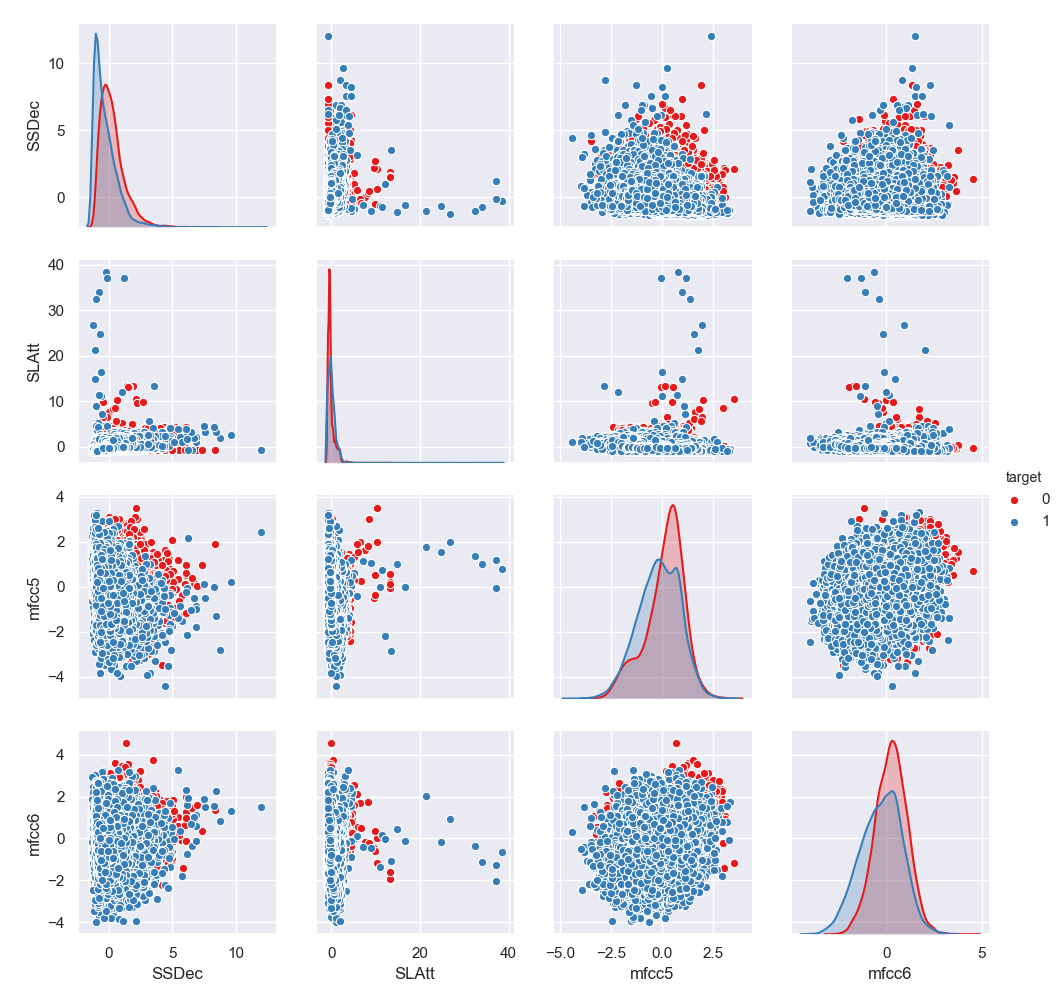
\includegraphics[width=0.7\textwidth]{figure_1.png}
\end{figure}
\begin{figure}[h]
\centering
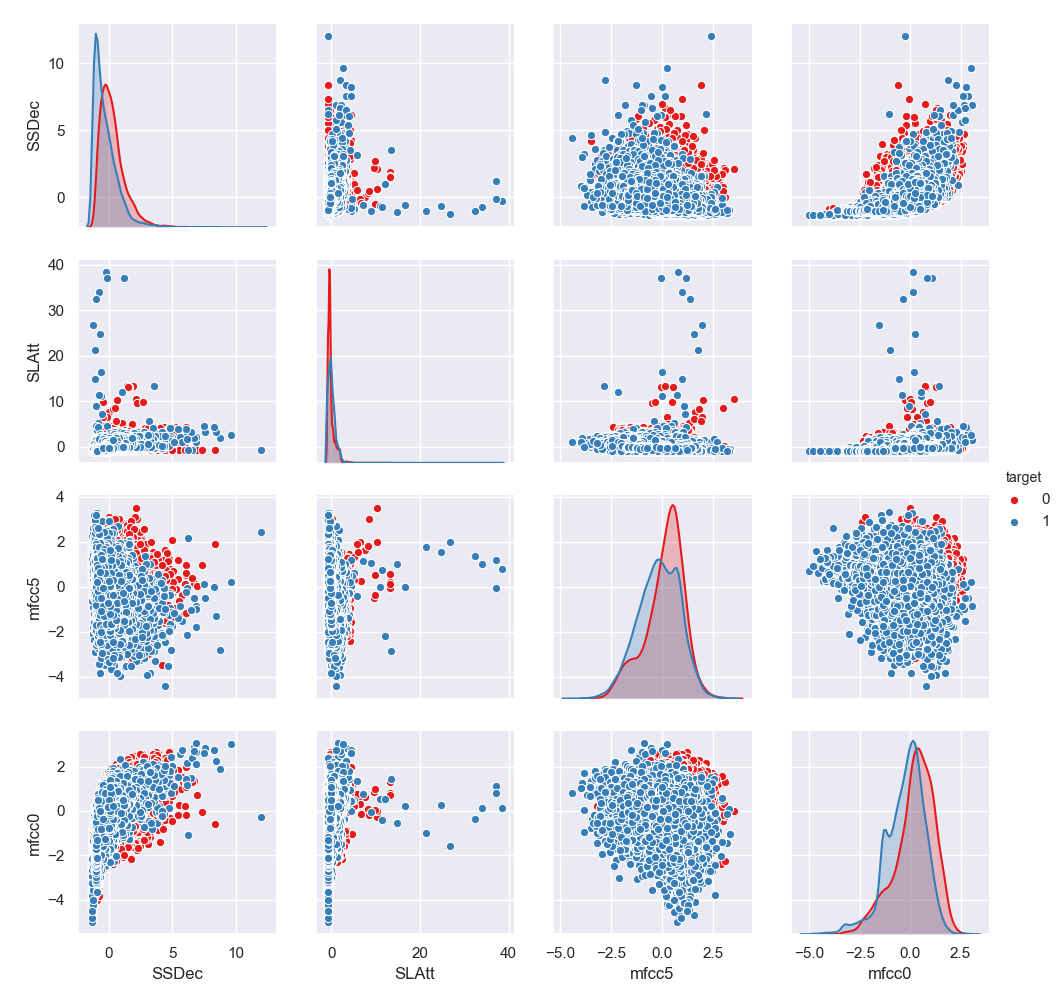
\includegraphics[width=0.7\textwidth]{figure_2.png}
\end{figure}


Eπιπλέον, ελέγξαμε όλα τα χαρακτηριστικά ένα προς ένα έτσι ώστε να δούμε εάν υπάρχει τρόπος να φτάσουμε την πλήρη ακρίβεια του μοντέλου μας με λιγότερα ή να φτάσουμε αρκετά κοντά ίσως ακόμα και με μόνο ένα. 
Tα αποτελέσματα έδειξαν ότι κανένα χαρακτηριστικό από μόνο του δεν είναι ικανό να δώσει ικανοποιητικό ποσοστό απόδοσης στο μοντέλο. Αν πάρουμε το καλύτερο feature και το δοκιμάσουμε σε συνδυασμό με τα υπόλοιπα βλέπουμε ότι η ακρίβεια αυξάνεται λίγο αλλά όχι αρκετά.  
Τέλος, αν συνδυάσουμε ξανά αυτά τα features που δίνουν το καλύτερο αποτέλεσμα βλέπουμε ότι έχουμε και πάλι μια μικρή αύξηση στην ακρίβεια ,η οποία όμως είναι αρκετά μακρυά από την ακρίβεια που πετυχαίνουμε εν τέλει. 

\begin{table}[h]
\begin{tabular}{llll}
{\ul \textbf{Accuracy}} & {\ul \textbf{Individually}} & {\ul \textbf{with best 1}} & {\ul \textbf{with best 2}} \\
4Hz Mod                 & 0.58                        & 0.66                       & 0.73                       \\
Flat                    & 0.63                        & 0.71                       & 0.75                       \\
HFC                     & 0.58                        & 0.65                       & 0.72                       \\
LAtt                    & 0.62                        & 0.71                       & 0.75                       \\
SC                      & 0.59                        & 0.66                       & 0.73                       \\
Scomp                   & 0.57                        & 0.66                       & 0.73                       \\
SDec                    & 0.63                        & 0.65                       & 0.72                       \\
SEFlat                  & 0.51                        & 0.65                       & 0.72                       \\
SF                      & 0.55                        & 0.69                       & 0.75                       \\
SFlat                   & 0.57                        & 0.66                       & 0.72                       \\
SLAtt                   & 0.63                        & 0.71                       & 0.74                       \\
SR                      & 0.60                        & 0.66                       & 0.72                       \\
SSDec                   & \textbf{0.65}               & -                          & -                          \\
ZCR                     & 0.58                        & 0.65                       & 0.72                       \\
mfcc0                   & 0.61                        & 0.66                       & 0.73                       \\
mfcc1                   & 0.58                        & 0.67                       & 0.73                       \\
mfcc2                   & 0.52                        & 0.66                       & 0.73                       \\
mfcc3                   & 0.56                        & 0.69                       & 0.76                       \\
mfcc4                   & 0.54                        & 0.67                       & 0.74                       \\
mfcc5                   & 0.57                        & 0.70                       & 0.75                       \\
mfcc6                   & 0.61                        & \textbf{0.72}              & -                          \\
mfcc7                   & 0.57                        & 0.68                       & 0.75                       \\
mfcc8                   & 0.55                        & 0.67                       & 0.74                       \\
mfcc9                   & 0.54                        & 0.67                       & 0.73                       \\
mfcc10                  & 0.54                        & 0.65                       & 0.73                       \\
mfcc11                  & 0.51                        & 0.66                       & 0.73                       \\
mfcc12                  & 0.54                        & 0.67                       & 0.73                      
\end{tabular}
\end{table}


Άρα, είναι προφανές ότι δεν είναι κάποιο συγκεκριμένο feature το οποίο ευθύνεται για το μεγαλύτερο ποσοστό της ακρίβειας του μοντέλου αλλά ο συνδυασμός τους.









